
\begin{frame}
	
	\frametitle{Evaluation of Proposed Approach }
	\framesubtitle{Selected Techniques}
	
	\begin{itemize}
		\item<1-> Theoretical Analysis. 
		
		\item<1-> Simulated synthetic data streams.
		
		\item<1->  Over real-world data streams of  AIS \footnote{AIS: \url{www.navcen.uscg.gov/?pageName=AISmain}} messages or derived trajectories critical points of moving vessels \citep{synopses1}. 
	\end{itemize}
	
\end{frame}

\begin{frame}
	
	\frametitle{ Evaluation of Proposed Approach }
	\framesubtitle{Performance Measures}

		\begin{itemize}
			\item<1->$\mathit{Precision = \frac{\#\ of\ correct\ predictions}{\#\ of\ total\ predictions}}$:
			 how many of the produced predictions are correct.  

 
			\item<1->  $\mathit{Recall = \frac{\#\ of\ full\ matches\ predicted\ at\ least\ once}{\#\ of\ total\ detected\ full\ matches}}$:
			 how many of the detected full matches of the defined pattern does the model predicate at least once in previous prediction. 
			
				\item<1->  $\mathit{Cumulative\ prediction\ loss}$:
		   aggregated number of all wrong predictions.
		\end{itemize}

\end{frame}



%\begin{frame}
%	
%	\frametitle{Initial Experimental Results }
%	\framesubtitle{Setup}
%1	analytical \& theoretical analysis 
% 2 evaluation with synthetic datastest \& 3 real datasets and grouping thing  
% then initial results 
%	
%\end{frame}


\begin{frame}
	
	\frametitle{Empirical evaluation }
	\framesubtitle{Experimental Setup}
\begin{itemize}
	\item<1-> Synopses over raw AIS messages in Brest, France: 1 October 2015 to 31 March 2016. 
	
	\item<1->$ 4,684,444$ derived critical points.
	
	\item<1->  $\approx5000$ vessels.
	\item<only@1> Used patterns: 
	$P_1=\mathit{change\_heading} \cdot \mathit{gap\_start} \cdot \mathit{gap\_end} \cdot 
	\mathit{change\_heading}$ or $\mathit{P_2=Sailing}$
\end{itemize}
	
\end{frame}


\begin{frame}
	
	\frametitle{Empirical evaluation }
	\framesubtitle{Initial  Results ($\mathit{P=Sailing}\ and\ batch\ size= 8)$}
	
	\begin{center}
		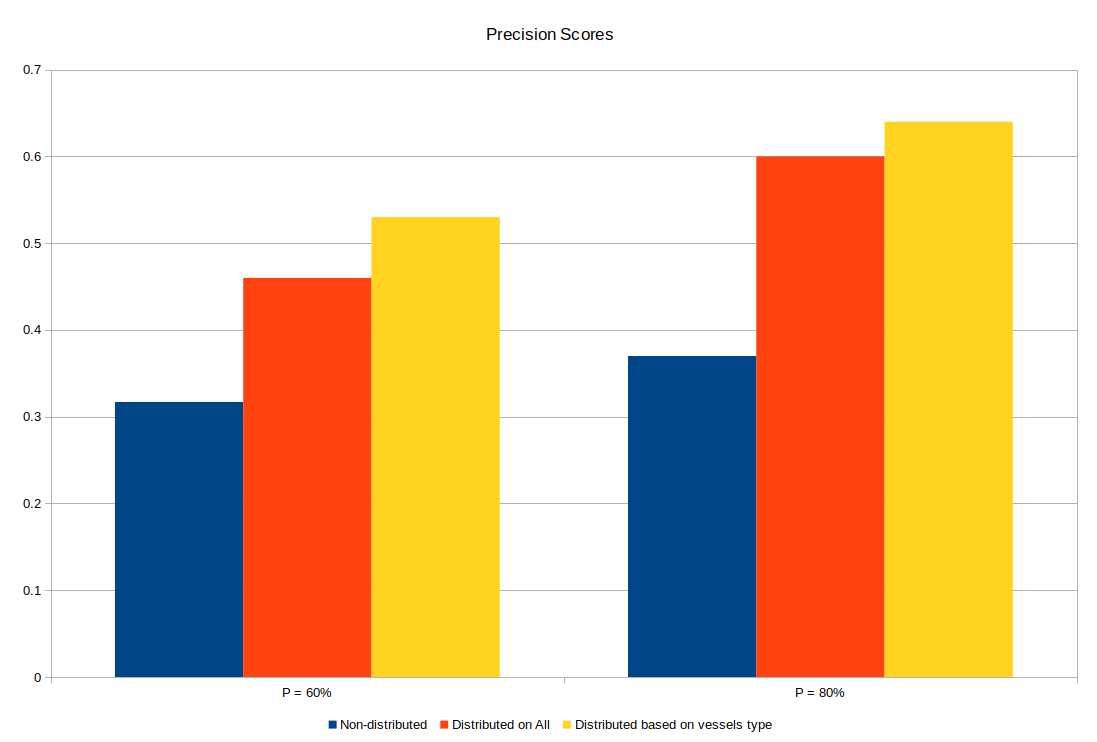
\includegraphics[width=1.05\textwidth,left]{figures/presention/precision_1.png}\\
		.
	\end{center}
	
\end{frame}


\begin{frame}
	
	\frametitle{Empirical evaluation }
	\framesubtitle{Initial  Results ($\mathit{P=Sailing}\ and\ batch\ size= 8)$}
	
	\begin{center}
		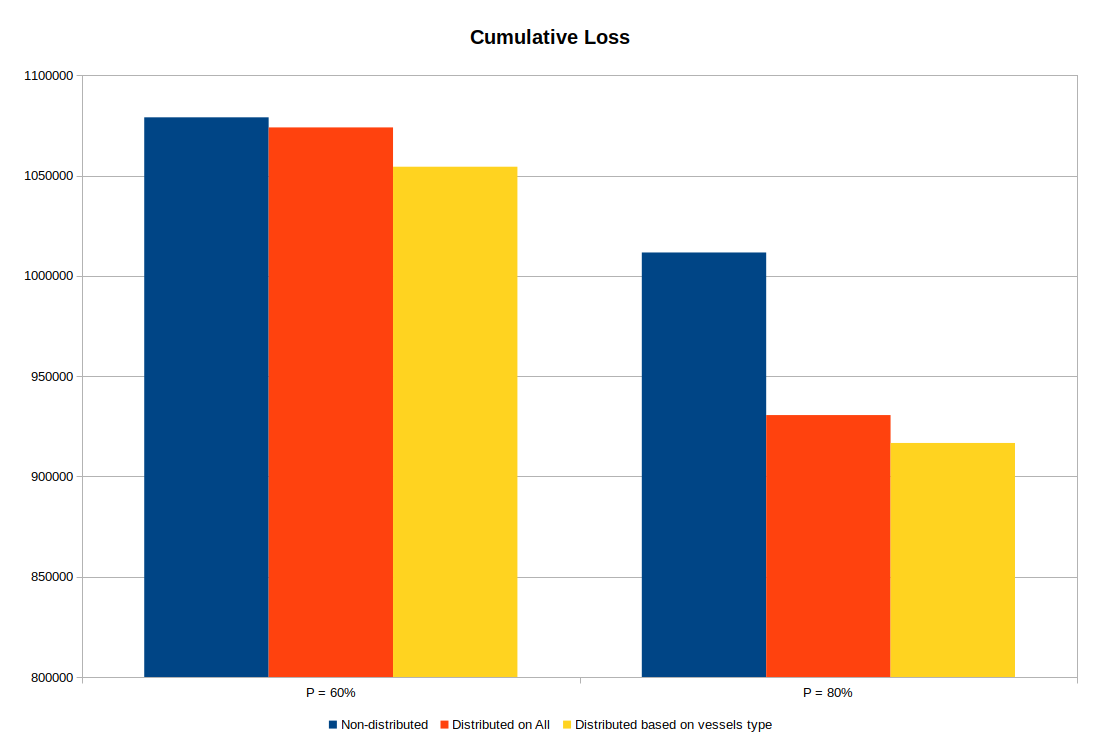
\includegraphics[width=1.05\textwidth,left]{figures/loss.png}\\
		.
	\end{center}
	
\end{frame}
%\begin{columns}
%	\begin{column}{0.5\textwidth}
%		\begin{itemize}
%			\item<1->Precision:
%			– how many of the produced predictions are correct
%		\end{itemize}
%	\end{column}
%	\begin{column}{0.5\textwidth}  %%<--- here
%		\begin{itemize}
%			\item<1->  Recall:
%			– how many of the full match does the model predicate at least once. 
%		\end{itemize}
%	\end{column}
%\end{columns}
%\end{frame}